\documentclass[1p]{elsarticle_modified}
%\bibliographystyle{elsarticle-num}

%\usepackage[colorlinks]{hyperref}
%\usepackage{abbrmath_seonhwa} %\Abb, \Ascr, \Acal ,\Abf, \Afrak
\usepackage{amsfonts}
\usepackage{amssymb}
\usepackage{amsmath}
\usepackage{amsthm}
\usepackage{scalefnt}
\usepackage{amsbsy}
\usepackage{kotex}
\usepackage{caption}
\usepackage{subfig}
\usepackage{color}
\usepackage{graphicx}
\usepackage{xcolor} %% white, black, red, green, blue, cyan, magenta, yellow
\usepackage{float}
\usepackage{setspace}
\usepackage{hyperref}

\usepackage{tikz}
\usetikzlibrary{arrows}

\usepackage{multirow}
\usepackage{array} % fixed length table
\usepackage{hhline}

%%%%%%%%%%%%%%%%%%%%%
\makeatletter
\renewcommand*\env@matrix[1][\arraystretch]{%
	\edef\arraystretch{#1}%
	\hskip -\arraycolsep
	\let\@ifnextchar\new@ifnextchar
	\array{*\c@MaxMatrixCols c}}
\makeatother %https://tex.stackexchange.com/questions/14071/how-can-i-increase-the-line-spacing-in-a-matrix
%%%%%%%%%%%%%%%

\usepackage[normalem]{ulem}

\newcommand{\msout}[1]{\ifmmode\text{\sout{\ensuremath{#1}}}\else\sout{#1}\fi}
%SOURCE: \msout is \stkout macro in https://tex.stackexchange.com/questions/20609/strikeout-in-math-mode

\newcommand{\cancel}[1]{
	\ifmmode
	{\color{red}\msout{#1}}
	\else
	{\color{red}\sout{#1}}
	\fi
}

\newcommand{\add}[1]{
	{\color{blue}\uwave{#1}}
}

\newcommand{\replace}[2]{
	\ifmmode
	{\color{red}\msout{#1}}{\color{blue}\uwave{#2}}
	\else
	{\color{red}\sout{#1}}{\color{blue}\uwave{#2}}
	\fi
}

\newcommand{\Sol}{\mathcal{S}} %segment
\newcommand{\D}{D} %diagram
\newcommand{\A}{\mathcal{A}} %arc


%%%%%%%%%%%%%%%%%%%%%%%%%%%%%5 test

\def\sl{\operatorname{\textup{SL}}(2,\Cbb)}
\def\psl{\operatorname{\textup{PSL}}(2,\Cbb)}
\def\quan{\mkern 1mu \triangleright \mkern 1mu}

\theoremstyle{definition}
\newtheorem{thm}{Theorem}[section]
\newtheorem{prop}[thm]{Proposition}
\newtheorem{lem}[thm]{Lemma}
\newtheorem{ques}[thm]{Question}
\newtheorem{cor}[thm]{Corollary}
\newtheorem{defn}[thm]{Definition}
\newtheorem{exam}[thm]{Example}
\newtheorem{rmk}[thm]{Remark}
\newtheorem{alg}[thm]{Algorithm}

\newcommand{\I}{\sqrt{-1}}
\begin{document}

%\begin{frontmatter}
%
%\title{Boundary parabolic representations of knots up to 8 crossings}
%
%%% Group authors per affiliation:
%\author{Yunhi Cho} 
%\address{Department of Mathematics, University of Seoul, Seoul, Korea}
%\ead{yhcho@uos.ac.kr}
%
%
%\author{Seonhwa Kim} %\fnref{s_kim}}
%\address{Center for Geometry and Physics, Institute for Basic Science, Pohang, 37673, Korea}
%\ead{ryeona17@ibs.re.kr}
%
%\author{Hyuk Kim}
%\address{Department of Mathematical Sciences, Seoul National University, Seoul 08826, Korea}
%\ead{hyukkim@snu.ac.kr}
%
%\author{Seokbeom Yoon}
%\address{Department of Mathematical Sciences, Seoul National University, Seoul, 08826,  Korea}
%\ead{sbyoon15@snu.ac.kr}
%
%\begin{abstract}
%We find all boundary parabolic representation of knots up to 8 crossings.
%
%\end{abstract}
%\begin{keyword}
%    \MSC[2010] 57M25 
%\end{keyword}
%
%\end{frontmatter}

%\linenumbers
%\tableofcontents
%
\newcommand\colored[1]{\textcolor{white}{\rule[-0.35ex]{0.8em}{1.4ex}}\kern-0.8em\color{red} #1}%
%\newcommand\colored[1]{\textcolor{white}{ #1}\kern-2.17ex	\textcolor{white}{ #1}\kern-1.81ex	\textcolor{white}{ #1}\kern-2.15ex\color{red}#1	}

{\Large $\underline{12a_{0592}~(K12a_{0592})}$}

\setlength{\tabcolsep}{10pt}
\renewcommand{\arraystretch}{1.6}
\vspace{1cm}\begin{tabular}{m{100pt}>{\centering\arraybackslash}m{274pt}}
\multirow{5}{120pt}{
	\centering
	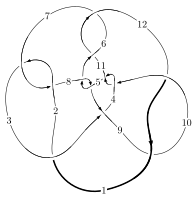
\includegraphics[width=112pt]{../../../GIT/diagram.site/Diagrams/png/1393_12a_0592.png}\\
\ \ \ A knot diagram\footnotemark}&
\allowdisplaybreaks
\textbf{Linearized knot diagam} \\
\cline{2-2}
 &
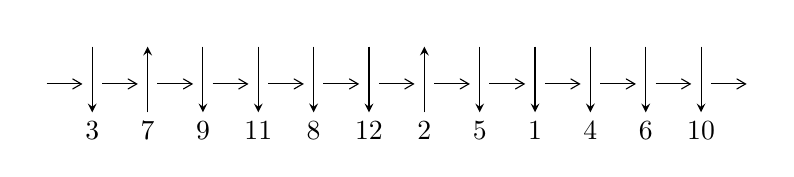
\begin{tikzpicture}[x=20pt, y=17pt]
	% nodes
	\node (C0) at (0, 0) {};
	\node (C1) at (1, 0) {};
	\node (C1U) at (1, +1) {};
	\node (C1D) at (1, -1) {3};

	\node (C2) at (2, 0) {};
	\node (C2U) at (2, +1) {};
	\node (C2D) at (2, -1) {7};

	\node (C3) at (3, 0) {};
	\node (C3U) at (3, +1) {};
	\node (C3D) at (3, -1) {9};

	\node (C4) at (4, 0) {};
	\node (C4U) at (4, +1) {};
	\node (C4D) at (4, -1) {11};

	\node (C5) at (5, 0) {};
	\node (C5U) at (5, +1) {};
	\node (C5D) at (5, -1) {8};

	\node (C6) at (6, 0) {};
	\node (C6U) at (6, +1) {};
	\node (C6D) at (6, -1) {12};

	\node (C7) at (7, 0) {};
	\node (C7U) at (7, +1) {};
	\node (C7D) at (7, -1) {2};

	\node (C8) at (8, 0) {};
	\node (C8U) at (8, +1) {};
	\node (C8D) at (8, -1) {5};

	\node (C9) at (9, 0) {};
	\node (C9U) at (9, +1) {};
	\node (C9D) at (9, -1) {1};

	\node (C10) at (10, 0) {};
	\node (C10U) at (10, +1) {};
	\node (C10D) at (10, -1) {4};

	\node (C11) at (11, 0) {};
	\node (C11U) at (11, +1) {};
	\node (C11D) at (11, -1) {6};

	\node (C12) at (12, 0) {};
	\node (C12U) at (12, +1) {};
	\node (C12D) at (12, -1) {10};
	\node (C13) at (13, 0) {};

	% arrows
	\draw[->,>={angle 60}]
	(C0) edge (C1) (C1) edge (C2) (C2) edge (C3) (C3) edge (C4) (C4) edge (C5) (C5) edge (C6) (C6) edge (C7) (C7) edge (C8) (C8) edge (C9) (C9) edge (C10) (C10) edge (C11) (C11) edge (C12) (C12) edge (C13) ;	\draw[->,>=stealth]
	(C1U) edge (C1D) (C2D) edge (C2U) (C3U) edge (C3D) (C4U) edge (C4D) (C5U) edge (C5D) (C6U) edge (C6D) (C7D) edge (C7U) (C8U) edge (C8D) (C9U) edge (C9D) (C10U) edge (C10D) (C11U) edge (C11D) (C12U) edge (C12D) ;
	\end{tikzpicture} \\
\hhline{~~} \\& 
\textbf{Solving Sequence} \\ \cline{2-2} 
 &
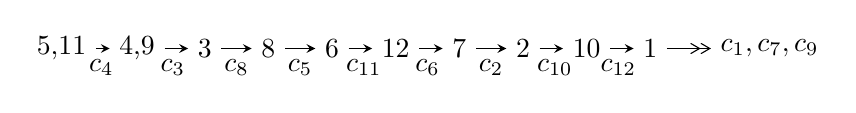
\begin{tikzpicture}[x=23pt, y=7pt]
	% node
	\node (A0) at (-1/8, 0) {5,11};
	\node (A1) at (17/16, 0) {4,9};
	\node (A2) at (17/8, 0) {3};
	\node (A3) at (25/8, 0) {8};
	\node (A4) at (33/8, 0) {6};
	\node (A5) at (41/8, 0) {12};
	\node (A6) at (49/8, 0) {7};
	\node (A7) at (57/8, 0) {2};
	\node (A8) at (65/8, 0) {10};
	\node (A9) at (73/8, 0) {1};
	\node (C1) at (1/2, -1) {$c_{4}$};
	\node (C2) at (13/8, -1) {$c_{3}$};
	\node (C3) at (21/8, -1) {$c_{8}$};
	\node (C4) at (29/8, -1) {$c_{5}$};
	\node (C5) at (37/8, -1) {$c_{11}$};
	\node (C6) at (45/8, -1) {$c_{6}$};
	\node (C7) at (53/8, -1) {$c_{2}$};
	\node (C8) at (61/8, -1) {$c_{10}$};
	\node (C9) at (69/8, -1) {$c_{12}$};
	\node (A10) at (11, 0) {$c_{1},c_{7},c_{9}$};

	% edge
	\draw[->,>=stealth]	
	(A0) edge (A1) (A1) edge (A2) (A2) edge (A3) (A3) edge (A4) (A4) edge (A5) (A5) edge (A6) (A6) edge (A7) (A7) edge (A8) (A8) edge (A9) ;
	\draw[->>,>={angle 60}]	
	(A9) edge (A10);
\end{tikzpicture} \\ 

\end{tabular} \\

\footnotetext{
The image of knot diagram is generated by the software ``\textbf{Draw programme}" developed by Andrew Bartholomew(\url{http://www.layer8.co.uk/maths/draw/index.htm\#Running-draw}), where we modified some parts for our purpose(\url{https://github.com/CATsTAILs/LinksPainter}).
}\phantom \\ \newline 
\centering \textbf{Ideals for irreducible components\footnotemark of $X_{\text{par}}$} 
 
\begin{align*}
I^u_{1}&=\langle 
1.27555\times10^{759} u^{147}-5.43746\times10^{758} u^{146}+\cdots+6.00623\times10^{760} b-3.19036\times10^{762},\\
\phantom{I^u_{1}}&\phantom{= \langle  }8.52310\times10^{761} u^{147}+2.29088\times10^{761} u^{146}+\cdots+5.65187\times10^{763} a+8.68018\times10^{766},\\
\phantom{I^u_{1}}&\phantom{= \langle  }u^{148}- u^{147}+\cdots-53808 u-30112\rangle \\
I^u_{2}&=\langle 
-9.48192\times10^{21} u^{39}-6.04550\times10^{22} u^{38}+\cdots+2.10677\times10^{21} b+4.56968\times10^{23},\\
\phantom{I^u_{2}}&\phantom{= \langle  }-1.41896\times10^{23} u^{39}-1.79678\times10^{23} u^{38}+\cdots+4.21354\times10^{21} a+1.49494\times10^{24},\\
\phantom{I^u_{2}}&\phantom{= \langle  }u^{40}-20 u^{38}+\cdots+14 u+4\rangle \\
\\
\end{align*}
\raggedright * 2 irreducible components of $\dim_{\mathbb{C}}=0$, with total 188 representations.\\
\footnotetext{All coefficients of polynomials are rational numbers. But the coefficients are sometimes approximated in decimal forms when there is not enough margin.}
\newpage
\renewcommand{\arraystretch}{1}
\centering \section*{I. $I^u_{1}= \langle 1.28\times10^{759} u^{147}-5.44\times10^{758} u^{146}+\cdots+6.01\times10^{760} b-3.19\times10^{762},\;8.52\times10^{761} u^{147}+2.29\times10^{761} u^{146}+\cdots+5.65\times10^{763} a+8.68\times10^{766},\;u^{148}- u^{147}+\cdots-53808 u-30112 \rangle$}
\flushleft \textbf{(i) Arc colorings}\\
\begin{tabular}{m{7pt} m{180pt} m{7pt} m{180pt} }
\flushright $a_{5}=$&$\begin{pmatrix}1\\0\end{pmatrix}$ \\
\flushright $a_{11}=$&$\begin{pmatrix}0\\u\end{pmatrix}$ \\
\flushright $a_{4}=$&$\begin{pmatrix}1\\- u^2\end{pmatrix}$ \\
\flushright $a_{9}=$&$\begin{pmatrix}-0.0150802 u^{147}-0.00405332 u^{146}+\cdots-3656.00 u-1535.81\\-0.0212371 u^{147}+0.00905302 u^{146}+\cdots-333.345 u+53.1175\end{pmatrix}$ \\
\flushright $a_{3}=$&$\begin{pmatrix}-0.0453474 u^{147}+0.00568426 u^{146}+\cdots-4034.83 u-1287.00\\0.00445966 u^{147}-0.0147265 u^{146}+\cdots+300.481 u-171.603\end{pmatrix}$ \\
\flushright $a_{8}=$&$\begin{pmatrix}-0.0363173 u^{147}+0.00499971 u^{146}+\cdots-3989.34 u-1482.69\\-0.0212371 u^{147}+0.00905302 u^{146}+\cdots-333.345 u+53.1175\end{pmatrix}$ \\
\flushright $a_{6}=$&$\begin{pmatrix}-0.00892067 u^{147}+0.0248161 u^{146}+\cdots+378.690 u+566.031\\0.00778258 u^{147}-0.00321811 u^{146}+\cdots-407.207 u-169.594\end{pmatrix}$ \\
\flushright $a_{12}=$&$\begin{pmatrix}0.0106950 u^{147}+0.00827467 u^{146}+\cdots+1227.05 u+759.853\\-0.00632593 u^{147}-0.00124789 u^{146}+\cdots-1576.14 u-566.286\end{pmatrix}$ \\
\flushright $a_{7}=$&$\begin{pmatrix}-0.0251779 u^{147}-0.000230073 u^{146}+\cdots-2451.98 u-1066.55\\0.0217830 u^{147}-0.000817469 u^{146}+\cdots+2049.68 u+830.946\end{pmatrix}$ \\
\flushright $a_{2}=$&$\begin{pmatrix}-0.0131109 u^{147}+0.0460703 u^{146}+\cdots+1069.10 u+1438.34\\-0.00169074 u^{147}-0.00435045 u^{146}+\cdots-1421.28 u-586.173\end{pmatrix}$ \\
\flushright $a_{10}=$&$\begin{pmatrix}u\\- u^3+u\end{pmatrix}$ \\
\flushright $a_{1}=$&$\begin{pmatrix}0.0127957 u^{147}+0.0131225 u^{146}+\cdots+1958.07 u+1128.43\\-0.00684151 u^{147}+0.000982730 u^{146}+\cdots-1282.27 u-406.943\end{pmatrix}$\\&\end{tabular}
\flushleft \textbf{(ii) Obstruction class $= -1$}\\~\\
\flushleft \textbf{(iii) Cusp Shapes $= 0.0629200 u^{147}-0.0215940 u^{146}+\cdots+2591.46 u+883.134$}\\~\\
\newpage\renewcommand{\arraystretch}{1}
\flushleft \textbf{(iv) u-Polynomials at the component}\newline \\
\begin{tabular}{m{50pt}|m{274pt}}
Crossings & \hspace{64pt}u-Polynomials at each crossing \\
\hline $$\begin{aligned}c_{1}\end{aligned}$$&$\begin{aligned}
&u^{148}+61 u^{147}+\cdots-482592 u+289
\end{aligned}$\\
\hline $$\begin{aligned}c_{2},c_{7}\end{aligned}$$&$\begin{aligned}
&u^{148}+u^{147}+\cdots+756 u-17
\end{aligned}$\\
\hline $$\begin{aligned}c_{3}\end{aligned}$$&$\begin{aligned}
&u^{148}+u^{147}+\cdots+218802202 u-23765389
\end{aligned}$\\
\hline $$\begin{aligned}c_{4},c_{10}\end{aligned}$$&$\begin{aligned}
&u^{148}- u^{147}+\cdots-53808 u-30112
\end{aligned}$\\
\hline $$\begin{aligned}c_{5},c_{8}\end{aligned}$$&$\begin{aligned}
&u^{148}-3 u^{147}+\cdots-2 u+1
\end{aligned}$\\
\hline $$\begin{aligned}c_{6},c_{11}\end{aligned}$$&$\begin{aligned}
&u^{148}+u^{147}+\cdots+72727 u-63873
\end{aligned}$\\
\hline $$\begin{aligned}c_{9},c_{12}\end{aligned}$$&$\begin{aligned}
&u^{148}-3 u^{147}+\cdots+27474 u-19583
\end{aligned}$\\
\hline
\end{tabular}\\~\\
\newpage\renewcommand{\arraystretch}{1}
\flushleft \textbf{(v) Riley Polynomials at the component}\newline \\
\begin{tabular}{m{50pt}|m{274pt}}
Crossings & \hspace{64pt}Riley Polynomials at each crossing \\
\hline $$\begin{aligned}c_{1}\end{aligned}$$&$\begin{aligned}
&y^{148}+73 y^{147}+\cdots-238131873368 y+83521
\end{aligned}$\\
\hline $$\begin{aligned}c_{2},c_{7}\end{aligned}$$&$\begin{aligned}
&y^{148}+61 y^{147}+\cdots-482592 y+289
\end{aligned}$\\
\hline $$\begin{aligned}c_{3}\end{aligned}$$&$\begin{aligned}
&y^{148}+33 y^{147}+\cdots+2075029942090772 y+564793714321321
\end{aligned}$\\
\hline $$\begin{aligned}c_{4},c_{10}\end{aligned}$$&$\begin{aligned}
&y^{148}-103 y^{147}+\cdots-18411894016 y+906732544
\end{aligned}$\\
\hline $$\begin{aligned}c_{5},c_{8}\end{aligned}$$&$\begin{aligned}
&y^{148}+77 y^{147}+\cdots+6 y+1
\end{aligned}$\\
\hline $$\begin{aligned}c_{6},c_{11}\end{aligned}$$&$\begin{aligned}
&y^{148}-93 y^{147}+\cdots-115187567377 y+4079760129
\end{aligned}$\\
\hline $$\begin{aligned}c_{9},c_{12}\end{aligned}$$&$\begin{aligned}
&y^{148}+83 y^{147}+\cdots+12878707260 y+383493889
\end{aligned}$\\
\hline
\end{tabular}\\~\\
\newpage\flushleft \textbf{(vi) Complex Volumes and Cusp Shapes}
$$\begin{array}{c|c|c}  
\text{Solutions to }I^u_{1}& \I (\text{vol} + \sqrt{-1}CS) & \text{Cusp shape}\\
 \hline 
\begin{aligned}
u &= \phantom{-}0.214326 + 0.984152 I \\
a &= -0.413942 - 0.125164 I \\
b &= \phantom{-}0.125114 - 1.307210 I\end{aligned}
 & \phantom{-}8.92003 + 0.75788 I & \phantom{-0.000000 } 0 \\ \hline\begin{aligned}
u &= \phantom{-}0.214326 - 0.984152 I \\
a &= -0.413942 + 0.125164 I \\
b &= \phantom{-}0.125114 + 1.307210 I\end{aligned}
 & \phantom{-}8.92003 - 0.75788 I & \phantom{-0.000000 } 0 \\ \hline\begin{aligned}
u &= \phantom{-}0.875978 + 0.463305 I \\
a &= -1.37403 - 1.00103 I \\
b &= \phantom{-}0.418855 + 1.265100 I\end{aligned}
 & \phantom{-}4.92923 + 3.61563 I & \phantom{-0.000000 } 0 \\ \hline\begin{aligned}
u &= \phantom{-}0.875978 - 0.463305 I \\
a &= -1.37403 + 1.00103 I \\
b &= \phantom{-}0.418855 - 1.265100 I\end{aligned}
 & \phantom{-}4.92923 - 3.61563 I & \phantom{-0.000000 } 0 \\ \hline\begin{aligned}
u &= -0.728586 + 0.700156 I \\
a &= \phantom{-}1.53251 + 0.28888 I \\
b &= -0.726083 + 1.133350 I\end{aligned}
 & \phantom{-}4.26806 + 2.29976 I & \phantom{-0.000000 } 0 \\ \hline\begin{aligned}
u &= -0.728586 - 0.700156 I \\
a &= \phantom{-}1.53251 - 0.28888 I \\
b &= -0.726083 - 1.133350 I\end{aligned}
 & \phantom{-}4.26806 - 2.29976 I & \phantom{-0.000000 } 0 \\ \hline\begin{aligned}
u &= -0.951042 + 0.391347 I \\
a &= \phantom{-}1.42389 - 1.07644 I \\
b &= -0.599424 + 1.189260 I\end{aligned}
 & \phantom{-}4.98091 + 2.21212 I & \phantom{-0.000000 } 0 \\ \hline\begin{aligned}
u &= -0.951042 - 0.391347 I \\
a &= \phantom{-}1.42389 + 1.07644 I \\
b &= -0.599424 - 1.189260 I\end{aligned}
 & \phantom{-}4.98091 - 2.21212 I & \phantom{-0.000000 } 0 \\ \hline\begin{aligned}
u &= \phantom{-}0.616095 + 0.737967 I \\
a &= -0.599399 + 0.213597 I \\
b &= \phantom{-}0.605983 - 0.665926 I\end{aligned}
 & \phantom{-}3.24880 - 1.43352 I & \phantom{-0.000000 } 0 \\ \hline\begin{aligned}
u &= \phantom{-}0.616095 - 0.737967 I \\
a &= -0.599399 - 0.213597 I \\
b &= \phantom{-}0.605983 + 0.665926 I\end{aligned}
 & \phantom{-}3.24880 + 1.43352 I & \phantom{-0.000000 } 0\\
 \hline 
 \end{array}$$\newpage$$\begin{array}{c|c|c}  
\text{Solutions to }I^u_{1}& \I (\text{vol} + \sqrt{-1}CS) & \text{Cusp shape}\\
 \hline 
\begin{aligned}
u &= -0.249400 + 0.922126 I \\
a &= \phantom{-}0.234199 - 0.007156 I \\
b &= \phantom{-}0.486978 + 1.199110 I\end{aligned}
 & \phantom{-}0.18577 - 7.33775 I & \phantom{-0.000000 } 0 \\ \hline\begin{aligned}
u &= -0.249400 - 0.922126 I \\
a &= \phantom{-}0.234199 + 0.007156 I \\
b &= \phantom{-}0.486978 - 1.199110 I\end{aligned}
 & \phantom{-}0.18577 + 7.33775 I & \phantom{-0.000000 } 0 \\ \hline\begin{aligned}
u &= -0.896819 + 0.328504 I \\
a &= -1.262960 + 0.025626 I \\
b &= \phantom{-}0.060611 - 0.674689 I\end{aligned}
 & -0.692038 + 0.363451 I & \phantom{-0.000000 } 0 \\ \hline\begin{aligned}
u &= -0.896819 - 0.328504 I \\
a &= -1.262960 - 0.025626 I \\
b &= \phantom{-}0.060611 + 0.674689 I\end{aligned}
 & -0.692038 - 0.363451 I & \phantom{-0.000000 } 0 \\ \hline\begin{aligned}
u &= \phantom{-}0.666548 + 0.677478 I \\
a &= -0.666523 + 0.085489 I \\
b &= \phantom{-}0.433476 - 0.618221 I\end{aligned}
 & \phantom{-}3.25690 - 1.41552 I & \phantom{-0.000000 } 0 \\ \hline\begin{aligned}
u &= \phantom{-}0.666548 - 0.677478 I \\
a &= -0.666523 - 0.085489 I \\
b &= \phantom{-}0.433476 + 0.618221 I\end{aligned}
 & \phantom{-}3.25690 + 1.41552 I & \phantom{-0.000000 } 0 \\ \hline\begin{aligned}
u &= \phantom{-}1.037240 + 0.227779 I \\
a &= \phantom{-}1.50158 - 0.50954 I \\
b &= -1.46327 + 0.47624 I\end{aligned}
 & -4.23688 + 0.02542 I & \phantom{-0.000000 } 0 \\ \hline\begin{aligned}
u &= \phantom{-}1.037240 - 0.227779 I \\
a &= \phantom{-}1.50158 + 0.50954 I \\
b &= -1.46327 - 0.47624 I\end{aligned}
 & -4.23688 - 0.02542 I & \phantom{-0.000000 } 0 \\ \hline\begin{aligned}
u &= -0.662915 + 0.641650 I \\
a &= -0.072510 - 0.271082 I \\
b &= -0.299940 - 1.036200 I\end{aligned}
 & \phantom{-}1.60102 - 1.05149 I & \phantom{-0.000000 } 0 \\ \hline\begin{aligned}
u &= -0.662915 - 0.641650 I \\
a &= -0.072510 + 0.271082 I \\
b &= -0.299940 + 1.036200 I\end{aligned}
 & \phantom{-}1.60102 + 1.05149 I & \phantom{-0.000000 } 0\\
 \hline 
 \end{array}$$\newpage$$\begin{array}{c|c|c}  
\text{Solutions to }I^u_{1}& \I (\text{vol} + \sqrt{-1}CS) & \text{Cusp shape}\\
 \hline 
\begin{aligned}
u &= \phantom{-}0.888829 + 0.173429 I \\
a &= -1.99544 + 0.85848 I \\
b &= \phantom{-}0.493308 + 1.059540 I\end{aligned}
 & -3.06656 - 6.30605 I & \phantom{-0.000000 } 0 \\ \hline\begin{aligned}
u &= \phantom{-}0.888829 - 0.173429 I \\
a &= -1.99544 - 0.85848 I \\
b &= \phantom{-}0.493308 - 1.059540 I\end{aligned}
 & -3.06656 + 6.30605 I & \phantom{-0.000000 } 0 \\ \hline\begin{aligned}
u &= \phantom{-}0.511896 + 0.969843 I \\
a &= -0.157976 + 0.616360 I \\
b &= \phantom{-}0.392535 + 0.963915 I\end{aligned}
 & -2.61321 + 0.25611 I & \phantom{-0.000000 } 0 \\ \hline\begin{aligned}
u &= \phantom{-}0.511896 - 0.969843 I \\
a &= -0.157976 - 0.616360 I \\
b &= \phantom{-}0.392535 - 0.963915 I\end{aligned}
 & -2.61321 - 0.25611 I & \phantom{-0.000000 } 0 \\ \hline\begin{aligned}
u &= \phantom{-}1.091240 + 0.136632 I \\
a &= \phantom{-}1.61954 + 0.32904 I \\
b &= -0.717318 - 0.658374 I\end{aligned}
 & -3.94319 - 2.68174 I & \phantom{-0.000000 } 0 \\ \hline\begin{aligned}
u &= \phantom{-}1.091240 - 0.136632 I \\
a &= \phantom{-}1.61954 - 0.32904 I \\
b &= -0.717318 + 0.658374 I\end{aligned}
 & -3.94319 + 2.68174 I & \phantom{-0.000000 } 0 \\ \hline\begin{aligned}
u &= \phantom{-}0.895060 + 0.040483 I \\
a &= -1.21100 + 0.90504 I \\
b &= \phantom{-}0.368272 + 1.140510 I\end{aligned}
 & -3.32363 + 2.05649 I & \phantom{-0.000000 } 0 \\ \hline\begin{aligned}
u &= \phantom{-}0.895060 - 0.040483 I \\
a &= -1.21100 - 0.90504 I \\
b &= \phantom{-}0.368272 - 1.140510 I\end{aligned}
 & -3.32363 - 2.05649 I & \phantom{-0.000000 } 0 \\ \hline\begin{aligned}
u &= -1.056220 + 0.343146 I \\
a &= -1.37535 - 0.67389 I \\
b &= \phantom{-}1.39335 + 0.63287 I\end{aligned}
 & -5.29713 + 5.12679 I & \phantom{-0.000000 } 0 \\ \hline\begin{aligned}
u &= -1.056220 - 0.343146 I \\
a &= -1.37535 + 0.67389 I \\
b &= \phantom{-}1.39335 - 0.63287 I\end{aligned}
 & -5.29713 - 5.12679 I & \phantom{-0.000000 } 0\\
 \hline 
 \end{array}$$\newpage$$\begin{array}{c|c|c}  
\text{Solutions to }I^u_{1}& \I (\text{vol} + \sqrt{-1}CS) & \text{Cusp shape}\\
 \hline 
\begin{aligned}
u &= \phantom{-}0.825724 + 0.747298 I \\
a &= -1.62385 + 0.23078 I \\
b &= \phantom{-}0.824376 + 1.057590 I\end{aligned}
 & \phantom{-}4.04498 - 7.25792 I & \phantom{-0.000000 } 0 \\ \hline\begin{aligned}
u &= \phantom{-}0.825724 - 0.747298 I \\
a &= -1.62385 - 0.23078 I \\
b &= \phantom{-}0.824376 - 1.057590 I\end{aligned}
 & \phantom{-}4.04498 + 7.25792 I & \phantom{-0.000000 } 0 \\ \hline\begin{aligned}
u &= -0.937222 + 0.604861 I \\
a &= \phantom{-}1.51139 + 0.80258 I \\
b &= -0.602775 + 0.275875 I\end{aligned}
 & \phantom{-}0.91085 + 8.01898 I & \phantom{-0.000000 } 0 \\ \hline\begin{aligned}
u &= -0.937222 - 0.604861 I \\
a &= \phantom{-}1.51139 - 0.80258 I \\
b &= -0.602775 - 0.275875 I\end{aligned}
 & \phantom{-}0.91085 - 8.01898 I & \phantom{-0.000000 } 0 \\ \hline\begin{aligned}
u &= \phantom{-}0.843385 + 0.201634 I \\
a &= -0.120544 + 0.790548 I \\
b &= \phantom{-}0.09359 - 1.82610 I\end{aligned}
 & \phantom{-}5.52470 - 6.41923 I & \phantom{-0.000000 } 0 \\ \hline\begin{aligned}
u &= \phantom{-}0.843385 - 0.201634 I \\
a &= -0.120544 - 0.790548 I \\
b &= \phantom{-}0.09359 + 1.82610 I\end{aligned}
 & \phantom{-}5.52470 + 6.41923 I & \phantom{-0.000000 } 0 \\ \hline\begin{aligned}
u &= -0.123533 + 0.856619 I \\
a &= \phantom{-}0.612379 - 0.162562 I \\
b &= -0.231194 - 1.354280 I\end{aligned}
 & \phantom{-}7.76303 - 6.83821 I & \phantom{-0.000000 } 0 \\ \hline\begin{aligned}
u &= -0.123533 - 0.856619 I \\
a &= \phantom{-}0.612379 + 0.162562 I \\
b &= -0.231194 + 1.354280 I\end{aligned}
 & \phantom{-}7.76303 + 6.83821 I & \phantom{-0.000000 } 0 \\ \hline\begin{aligned}
u &= \phantom{-}0.667705 + 0.546943 I \\
a &= \phantom{-}0.885097 - 0.534374 I \\
b &= \phantom{-}0.343696 - 0.601604 I\end{aligned}
 & -3.48032 + 3.66211 I & \phantom{-0.000000 } 0 \\ \hline\begin{aligned}
u &= \phantom{-}0.667705 - 0.546943 I \\
a &= \phantom{-}0.885097 + 0.534374 I \\
b &= \phantom{-}0.343696 + 0.601604 I\end{aligned}
 & -3.48032 - 3.66211 I & \phantom{-0.000000 } 0\\
 \hline 
 \end{array}$$\newpage$$\begin{array}{c|c|c}  
\text{Solutions to }I^u_{1}& \I (\text{vol} + \sqrt{-1}CS) & \text{Cusp shape}\\
 \hline 
\begin{aligned}
u &= -1.137020 + 0.145280 I \\
a &= -1.199480 - 0.623228 I \\
b &= \phantom{-}0.289719 - 1.106420 I\end{aligned}
 & -3.22971 + 2.24180 I & \phantom{-0.000000 } 0 \\ \hline\begin{aligned}
u &= -1.137020 - 0.145280 I \\
a &= -1.199480 + 0.623228 I \\
b &= \phantom{-}0.289719 + 1.106420 I\end{aligned}
 & -3.22971 - 2.24180 I & \phantom{-0.000000 } 0 \\ \hline\begin{aligned}
u &= -0.826873 + 0.171169 I \\
a &= \phantom{-}0.540158 + 0.720506 I \\
b &= -0.30509 - 1.76458 I\end{aligned}
 & \phantom{-}5.83530 + 0.18265 I & \phantom{-0.000000 } 0 \\ \hline\begin{aligned}
u &= -0.826873 - 0.171169 I \\
a &= \phantom{-}0.540158 - 0.720506 I \\
b &= -0.30509 + 1.76458 I\end{aligned}
 & \phantom{-}5.83530 - 0.18265 I & \phantom{-0.000000 } 0 \\ \hline\begin{aligned}
u &= \phantom{-}0.714796 + 0.443811 I \\
a &= -1.72520 + 0.66537 I \\
b &= \phantom{-}0.174414 - 0.264431 I\end{aligned}
 & \phantom{-}2.95438 - 3.17982 I & \phantom{-0.000000 } 0 \\ \hline\begin{aligned}
u &= \phantom{-}0.714796 - 0.443811 I \\
a &= -1.72520 - 0.66537 I \\
b &= \phantom{-}0.174414 + 0.264431 I\end{aligned}
 & \phantom{-}2.95438 + 3.17982 I & \phantom{-0.000000 } 0 \\ \hline\begin{aligned}
u &= \phantom{-}0.814438 + 0.189957 I \\
a &= \phantom{-}2.49440 - 0.42645 I \\
b &= -1.234240 + 0.009765 I\end{aligned}
 & -3.36046 - 1.80092 I & \phantom{-0.000000 } 0 \\ \hline\begin{aligned}
u &= \phantom{-}0.814438 - 0.189957 I \\
a &= \phantom{-}2.49440 + 0.42645 I \\
b &= -1.234240 - 0.009765 I\end{aligned}
 & -3.36046 + 1.80092 I & \phantom{-0.000000 } 0 \\ \hline\begin{aligned}
u &= \phantom{-}0.804465 + 0.844735 I \\
a &= -0.170498 + 0.539610 I \\
b &= \phantom{-}0.581615 - 1.172870 I\end{aligned}
 & \phantom{-}4.16225 + 1.37790 I & \phantom{-0.000000 } 0 \\ \hline\begin{aligned}
u &= \phantom{-}0.804465 - 0.844735 I \\
a &= -0.170498 - 0.539610 I \\
b &= \phantom{-}0.581615 + 1.172870 I\end{aligned}
 & \phantom{-}4.16225 - 1.37790 I & \phantom{-0.000000 } 0\\
 \hline 
 \end{array}$$\newpage$$\begin{array}{c|c|c}  
\text{Solutions to }I^u_{1}& \I (\text{vol} + \sqrt{-1}CS) & \text{Cusp shape}\\
 \hline 
\begin{aligned}
u &= -1.077740 + 0.455945 I \\
a &= \phantom{-}1.87684 - 0.06520 I \\
b &= -0.525181 + 1.024050 I\end{aligned}
 & \phantom{-}0.20875 + 5.40054 I & \phantom{-0.000000 } 0 \\ \hline\begin{aligned}
u &= -1.077740 - 0.455945 I \\
a &= \phantom{-}1.87684 + 0.06520 I \\
b &= -0.525181 - 1.024050 I\end{aligned}
 & \phantom{-}0.20875 - 5.40054 I & \phantom{-0.000000 } 0 \\ \hline\begin{aligned}
u &= -0.863979 + 0.796330 I \\
a &= -0.046595 + 0.541979 I \\
b &= -0.455481 - 1.231400 I\end{aligned}
 & \phantom{-}3.95808 + 3.32044 I & \phantom{-0.000000 } 0 \\ \hline\begin{aligned}
u &= -0.863979 - 0.796330 I \\
a &= -0.046595 - 0.541979 I \\
b &= -0.455481 + 1.231400 I\end{aligned}
 & \phantom{-}3.95808 - 3.32044 I & \phantom{-0.000000 } 0 \\ \hline\begin{aligned}
u &= -0.009550 + 1.181060 I \\
a &= -0.006924 + 0.467320 I \\
b &= \phantom{-}0.404163 + 0.873428 I\end{aligned}
 & -2.67414 + 0.10161 I & \phantom{-0.000000 } 0 \\ \hline\begin{aligned}
u &= -0.009550 - 1.181060 I \\
a &= -0.006924 - 0.467320 I \\
b &= \phantom{-}0.404163 - 0.873428 I\end{aligned}
 & -2.67414 - 0.10161 I & \phantom{-0.000000 } 0 \\ \hline\begin{aligned}
u &= -0.426735 + 0.696337 I \\
a &= \phantom{-}0.648366 + 0.204756 I \\
b &= -0.806994 - 0.353529 I\end{aligned}
 & \phantom{-}2.33256 - 3.28873 I & \phantom{-0.000000 } 0 \\ \hline\begin{aligned}
u &= -0.426735 - 0.696337 I \\
a &= \phantom{-}0.648366 - 0.204756 I \\
b &= -0.806994 + 0.353529 I\end{aligned}
 & \phantom{-}2.33256 + 3.28873 I & \phantom{-0.000000 } 0 \\ \hline\begin{aligned}
u &= \phantom{-}0.971663 + 0.692788 I \\
a &= -1.62485 + 0.41674 I \\
b &= \phantom{-}0.745783 + 0.686738 I\end{aligned}
 & \phantom{-}2.32462 - 4.03949 I & \phantom{-0.000000 } 0 \\ \hline\begin{aligned}
u &= \phantom{-}0.971663 - 0.692788 I \\
a &= -1.62485 - 0.41674 I \\
b &= \phantom{-}0.745783 - 0.686738 I\end{aligned}
 & \phantom{-}2.32462 + 4.03949 I & \phantom{-0.000000 } 0\\
 \hline 
 \end{array}$$\newpage$$\begin{array}{c|c|c}  
\text{Solutions to }I^u_{1}& \I (\text{vol} + \sqrt{-1}CS) & \text{Cusp shape}\\
 \hline 
\begin{aligned}
u &= -0.712291 + 0.369817 I \\
a &= \phantom{-}2.33356 + 1.23617 I \\
b &= -0.099743 - 0.239624 I\end{aligned}
 & \phantom{-}1.10383 + 8.13108 I & \phantom{-0.000000 } 0 \\ \hline\begin{aligned}
u &= -0.712291 - 0.369817 I \\
a &= \phantom{-}2.33356 - 1.23617 I \\
b &= -0.099743 + 0.239624 I\end{aligned}
 & \phantom{-}1.10383 - 8.13108 I & \phantom{-0.000000 } 0 \\ \hline\begin{aligned}
u &= -0.794476 + 0.106943 I \\
a &= \phantom{-}1.72375 + 0.60210 I \\
b &= -0.505956 + 1.138630 I\end{aligned}
 & \phantom{-}0.32935 + 2.06920 I & \phantom{-0.000000 } 0 \\ \hline\begin{aligned}
u &= -0.794476 - 0.106943 I \\
a &= \phantom{-}1.72375 - 0.60210 I \\
b &= -0.505956 - 1.138630 I\end{aligned}
 & \phantom{-}0.32935 - 2.06920 I & \phantom{-0.000000 } 0 \\ \hline\begin{aligned}
u &= \phantom{-}1.163500 + 0.302367 I \\
a &= \phantom{-}1.227760 + 0.031436 I \\
b &= -0.473347 - 1.278390 I\end{aligned}
 & -1.19171 - 5.50814 I & \phantom{-0.000000 } 0 \\ \hline\begin{aligned}
u &= \phantom{-}1.163500 - 0.302367 I \\
a &= \phantom{-}1.227760 - 0.031436 I \\
b &= -0.473347 + 1.278390 I\end{aligned}
 & -1.19171 + 5.50814 I & \phantom{-0.000000 } 0 \\ \hline\begin{aligned}
u &= \phantom{-}0.267676 + 0.749235 I \\
a &= -0.637894 + 0.129383 I \\
b &= -0.325619 + 1.165970 I\end{aligned}
 & \phantom{-}1.78491 + 2.49380 I & \phantom{-0.000000 } 0 \\ \hline\begin{aligned}
u &= \phantom{-}0.267676 - 0.749235 I \\
a &= -0.637894 - 0.129383 I \\
b &= -0.325619 - 1.165970 I\end{aligned}
 & \phantom{-}1.78491 - 2.49380 I & \phantom{-0.000000 } 0 \\ \hline\begin{aligned}
u &= \phantom{-}1.223360 + 0.088706 I \\
a &= -0.564615 - 1.141070 I \\
b &= \phantom{-}0.507809 + 0.485334 I\end{aligned}
 & -4.81534 + 2.14628 I & \phantom{-0.000000 } 0 \\ \hline\begin{aligned}
u &= \phantom{-}1.223360 - 0.088706 I \\
a &= -0.564615 + 1.141070 I \\
b &= \phantom{-}0.507809 - 0.485334 I\end{aligned}
 & -4.81534 - 2.14628 I & \phantom{-0.000000 } 0\\
 \hline 
 \end{array}$$\newpage$$\begin{array}{c|c|c}  
\text{Solutions to }I^u_{1}& \I (\text{vol} + \sqrt{-1}CS) & \text{Cusp shape}\\
 \hline 
\begin{aligned}
u &= \phantom{-}1.22763\phantom{ +0.000000I} \\
a &= \phantom{-}1.26399\phantom{ +0.000000I} \\
b &= -1.14801\phantom{ +0.000000I}\end{aligned}
 & -5.55891\phantom{ +0.000000I} & \phantom{-0.000000 } 0 \\ \hline\begin{aligned}
u &= -1.159340 + 0.410415 I \\
a &= -1.256630 + 0.541922 I \\
b &= \phantom{-}0.329053 - 1.154260 I\end{aligned}
 & \phantom{-}1.42778 + 1.54612 I & \phantom{-0.000000 } 0 \\ \hline\begin{aligned}
u &= -1.159340 - 0.410415 I \\
a &= -1.256630 - 0.541922 I \\
b &= \phantom{-}0.329053 + 1.154260 I\end{aligned}
 & \phantom{-}1.42778 - 1.54612 I & \phantom{-0.000000 } 0 \\ \hline\begin{aligned}
u &= -0.051071 + 0.763432 I \\
a &= \phantom{-}0.107953 + 0.396029 I \\
b &= -0.081193 + 1.297080 I\end{aligned}
 & \phantom{-}4.70452 + 2.64087 I & \phantom{-0.000000 } 0 \\ \hline\begin{aligned}
u &= -0.051071 - 0.763432 I \\
a &= \phantom{-}0.107953 - 0.396029 I \\
b &= -0.081193 - 1.297080 I\end{aligned}
 & \phantom{-}4.70452 - 2.64087 I & \phantom{-0.000000 } 0 \\ \hline\begin{aligned}
u &= -1.253150 + 0.243833 I \\
a &= \phantom{-}0.820966 - 0.523948 I \\
b &= -0.743124 + 0.209233 I\end{aligned}
 & -2.39226 + 2.63611 I & \phantom{-0.000000 } 0 \\ \hline\begin{aligned}
u &= -1.253150 - 0.243833 I \\
a &= \phantom{-}0.820966 + 0.523948 I \\
b &= -0.743124 - 0.209233 I\end{aligned}
 & -2.39226 - 2.63611 I & \phantom{-0.000000 } 0 \\ \hline\begin{aligned}
u &= -0.648801 + 0.319269 I \\
a &= \phantom{-}0.76138 + 1.36805 I \\
b &= -0.320323 - 0.183103 I\end{aligned}
 & -1.48409 + 1.41052 I & \phantom{-0.000000 } 0 \\ \hline\begin{aligned}
u &= -0.648801 - 0.319269 I \\
a &= \phantom{-}0.76138 - 1.36805 I \\
b &= -0.320323 + 0.183103 I\end{aligned}
 & -1.48409 - 1.41052 I & \phantom{-0.000000 } 0 \\ \hline\begin{aligned}
u &= -1.273150 + 0.153104 I \\
a &= -1.90554 - 0.22647 I \\
b &= \phantom{-}0.529291 - 1.023470 I\end{aligned}
 & -2.37540 + 8.20990 I & \phantom{-0.000000 } 0\\
 \hline 
 \end{array}$$\newpage$$\begin{array}{c|c|c}  
\text{Solutions to }I^u_{1}& \I (\text{vol} + \sqrt{-1}CS) & \text{Cusp shape}\\
 \hline 
\begin{aligned}
u &= -1.273150 - 0.153104 I \\
a &= -1.90554 + 0.22647 I \\
b &= \phantom{-}0.529291 + 1.023470 I\end{aligned}
 & -2.37540 - 8.20990 I & \phantom{-0.000000 } 0 \\ \hline\begin{aligned}
u &= -0.704151 + 0.077832 I \\
a &= \phantom{-}1.77620 + 1.60667 I \\
b &= -0.245995 - 0.517858 I\end{aligned}
 & -1.43176 + 1.40849 I & \phantom{-0.000000 } 0 \\ \hline\begin{aligned}
u &= -0.704151 - 0.077832 I \\
a &= \phantom{-}1.77620 - 1.60667 I \\
b &= -0.245995 + 0.517858 I\end{aligned}
 & -1.43176 - 1.40849 I & \phantom{-0.000000 } 0 \\ \hline\begin{aligned}
u &= \phantom{-}1.237810 + 0.376131 I \\
a &= \phantom{-}1.39276 + 0.59417 I \\
b &= -0.461339 - 1.212050 I\end{aligned}
 & \phantom{-}0.79281 - 6.70296 I & \phantom{-0.000000 } 0 \\ \hline\begin{aligned}
u &= \phantom{-}1.237810 - 0.376131 I \\
a &= \phantom{-}1.39276 - 0.59417 I \\
b &= -0.461339 + 1.212050 I\end{aligned}
 & \phantom{-}0.79281 + 6.70296 I & \phantom{-0.000000 } 0 \\ \hline\begin{aligned}
u &= -1.241830 + 0.421803 I \\
a &= \phantom{-}1.292470 + 0.222253 I \\
b &= -1.249670 - 0.232251 I\end{aligned}
 & -0.90694 + 6.57296 I & \phantom{-0.000000 } 0 \\ \hline\begin{aligned}
u &= -1.241830 - 0.421803 I \\
a &= \phantom{-}1.292470 - 0.222253 I \\
b &= -1.249670 + 0.232251 I\end{aligned}
 & -0.90694 - 6.57296 I & \phantom{-0.000000 } 0 \\ \hline\begin{aligned}
u &= \phantom{-}1.298230 + 0.215686 I \\
a &= \phantom{-}1.77177 + 0.08749 I \\
b &= -0.583511 - 1.117650 I\end{aligned}
 & -1.41694 - 4.12322 I & \phantom{-0.000000 } 0 \\ \hline\begin{aligned}
u &= \phantom{-}1.298230 - 0.215686 I \\
a &= \phantom{-}1.77177 - 0.08749 I \\
b &= -0.583511 + 1.117650 I\end{aligned}
 & -1.41694 + 4.12322 I & \phantom{-0.000000 } 0 \\ \hline\begin{aligned}
u &= \phantom{-}1.209010 + 0.535306 I \\
a &= \phantom{-}1.41109 + 0.17868 I \\
b &= -0.72545 - 1.32288 I\end{aligned}
 & -1.13918 - 7.42902 I & \phantom{-0.000000 } 0\\
 \hline 
 \end{array}$$\newpage$$\begin{array}{c|c|c}  
\text{Solutions to }I^u_{1}& \I (\text{vol} + \sqrt{-1}CS) & \text{Cusp shape}\\
 \hline 
\begin{aligned}
u &= \phantom{-}1.209010 - 0.535306 I \\
a &= \phantom{-}1.41109 - 0.17868 I \\
b &= -0.72545 + 1.32288 I\end{aligned}
 & -1.13918 + 7.42902 I & \phantom{-0.000000 } 0 \\ \hline\begin{aligned}
u &= \phantom{-}1.255250 + 0.455390 I \\
a &= -1.304540 + 0.394555 I \\
b &= \phantom{-}1.286180 - 0.361410 I\end{aligned}
 & -2.43010 - 12.50910 I & \phantom{-0.000000 } 0 \\ \hline\begin{aligned}
u &= \phantom{-}1.255250 - 0.455390 I \\
a &= -1.304540 - 0.394555 I \\
b &= \phantom{-}1.286180 + 0.361410 I\end{aligned}
 & -2.43010 + 12.50910 I & \phantom{-0.000000 } 0 \\ \hline\begin{aligned}
u &= -0.616306 + 0.235557 I \\
a &= -2.85037 - 0.71023 I \\
b &= \phantom{-}1.201670 - 0.077763 I\end{aligned}
 & -3.66033 - 2.34896 I & -8.00000 + 0. I\phantom{ +0.000000I} \\ \hline\begin{aligned}
u &= -0.616306 - 0.235557 I \\
a &= -2.85037 + 0.71023 I \\
b &= \phantom{-}1.201670 + 0.077763 I\end{aligned}
 & -3.66033 + 2.34896 I & -8.00000 + 0. I\phantom{ +0.000000I} \\ \hline\begin{aligned}
u &= -1.320820 + 0.305987 I \\
a &= -0.970657 - 0.471871 I \\
b &= \phantom{-}0.994008 + 0.576575 I\end{aligned}
 & -8.66253 - 0.60401 I & \phantom{-0.000000 } 0 \\ \hline\begin{aligned}
u &= -1.320820 - 0.305987 I \\
a &= -0.970657 + 0.471871 I \\
b &= \phantom{-}0.994008 - 0.576575 I\end{aligned}
 & -8.66253 + 0.60401 I & \phantom{-0.000000 } 0 \\ \hline\begin{aligned}
u &= -1.229530 + 0.581363 I \\
a &= -1.51529 + 0.16255 I \\
b &= \phantom{-}0.80486 - 1.30600 I\end{aligned}
 & -2.82328 + 12.84140 I & \phantom{-0.000000 } 0 \\ \hline\begin{aligned}
u &= -1.229530 - 0.581363 I \\
a &= -1.51529 - 0.16255 I \\
b &= \phantom{-}0.80486 + 1.30600 I\end{aligned}
 & -2.82328 - 12.84140 I & \phantom{-0.000000 } 0 \\ \hline\begin{aligned}
u &= -0.081073 + 0.634388 I \\
a &= -0.57920 + 1.93892 I \\
b &= \phantom{-}0.667637 - 0.038832 I\end{aligned}
 & \phantom{-}1.39414 + 8.18526 I & -8.00000 - 6.02308 I\\
 \hline 
 \end{array}$$\newpage$$\begin{array}{c|c|c}  
\text{Solutions to }I^u_{1}& \I (\text{vol} + \sqrt{-1}CS) & \text{Cusp shape}\\
 \hline 
\begin{aligned}
u &= -0.081073 - 0.634388 I \\
a &= -0.57920 - 1.93892 I \\
b &= \phantom{-}0.667637 + 0.038832 I\end{aligned}
 & \phantom{-}1.39414 - 8.18526 I & -8.00000 + 6.02308 I \\ \hline\begin{aligned}
u &= \phantom{-}0.133983 + 1.370320 I \\
a &= -0.176285 - 0.077669 I \\
b &= \phantom{-}0.479349 - 1.177650 I\end{aligned}
 & \phantom{-}4.60946 + 12.50000 I & \phantom{-0.000000 } 0 \\ \hline\begin{aligned}
u &= \phantom{-}0.133983 - 1.370320 I \\
a &= -0.176285 + 0.077669 I \\
b &= \phantom{-}0.479349 + 1.177650 I\end{aligned}
 & \phantom{-}4.60946 - 12.50000 I & \phantom{-0.000000 } 0 \\ \hline\begin{aligned}
u &= \phantom{-}1.022250 + 0.927072 I \\
a &= -0.879569 + 0.239215 I \\
b &= \phantom{-}0.155848 + 0.747830 I\end{aligned}
 & \phantom{-}3.30780 - 3.79544 I & \phantom{-0.000000 } 0 \\ \hline\begin{aligned}
u &= \phantom{-}1.022250 - 0.927072 I \\
a &= -0.879569 - 0.239215 I \\
b &= \phantom{-}0.155848 - 0.747830 I\end{aligned}
 & \phantom{-}3.30780 + 3.79544 I & \phantom{-0.000000 } 0 \\ \hline\begin{aligned}
u &= \phantom{-}1.331330 + 0.381959 I \\
a &= -0.779290 + 0.250615 I \\
b &= \phantom{-}0.877413 - 0.342917 I\end{aligned}
 & -7.75176 - 5.15920 I & \phantom{-0.000000 } 0 \\ \hline\begin{aligned}
u &= \phantom{-}1.331330 - 0.381959 I \\
a &= -0.779290 - 0.250615 I \\
b &= \phantom{-}0.877413 + 0.342917 I\end{aligned}
 & -7.75176 + 5.15920 I & \phantom{-0.000000 } 0 \\ \hline\begin{aligned}
u &= -1.300680 + 0.483221 I \\
a &= \phantom{-}1.63652 - 0.62460 I \\
b &= -0.458365 + 1.149120 I\end{aligned}
 & \phantom{-}4.04375 + 11.79160 I & \phantom{-0.000000 } 0 \\ \hline\begin{aligned}
u &= -1.300680 - 0.483221 I \\
a &= \phantom{-}1.63652 + 0.62460 I \\
b &= -0.458365 - 1.149120 I\end{aligned}
 & \phantom{-}4.04375 - 11.79160 I & \phantom{-0.000000 } 0 \\ \hline\begin{aligned}
u &= \phantom{-}1.286990 + 0.557136 I \\
a &= -1.46980 - 0.51039 I \\
b &= \phantom{-}0.396994 + 1.115720 I\end{aligned}
 & \phantom{-}5.50576 - 6.31586 I & \phantom{-0.000000 } 0\\
 \hline 
 \end{array}$$\newpage$$\begin{array}{c|c|c}  
\text{Solutions to }I^u_{1}& \I (\text{vol} + \sqrt{-1}CS) & \text{Cusp shape}\\
 \hline 
\begin{aligned}
u &= \phantom{-}1.286990 - 0.557136 I \\
a &= -1.46980 + 0.51039 I \\
b &= \phantom{-}0.396994 - 1.115720 I\end{aligned}
 & \phantom{-}5.50576 + 6.31586 I & \phantom{-0.000000 } 0 \\ \hline\begin{aligned}
u &= \phantom{-}0.584949 + 0.076704 I \\
a &= \phantom{-}1.99785 + 0.94568 I \\
b &= \phantom{-}0.220757 - 0.047935 I\end{aligned}
 & -3.40808 - 3.41795 I & -12.5624 + 7.5263 I \\ \hline\begin{aligned}
u &= \phantom{-}0.584949 - 0.076704 I \\
a &= \phantom{-}1.99785 - 0.94568 I \\
b &= \phantom{-}0.220757 + 0.047935 I\end{aligned}
 & -3.40808 + 3.41795 I & -12.5624 - 7.5263 I \\ \hline\begin{aligned}
u &= -1.31304 + 0.52825 I \\
a &= -1.336860 - 0.058270 I \\
b &= \phantom{-}0.684439 - 1.154200 I\end{aligned}
 & -6.71138 + 5.53970 I & \phantom{-0.000000 } 0 \\ \hline\begin{aligned}
u &= -1.31304 - 0.52825 I \\
a &= -1.336860 + 0.058270 I \\
b &= \phantom{-}0.684439 + 1.154200 I\end{aligned}
 & -6.71138 - 5.53970 I & \phantom{-0.000000 } 0 \\ \hline\begin{aligned}
u &= \phantom{-}1.41796 + 0.06674 I \\
a &= \phantom{-}1.086540 - 0.564100 I \\
b &= -0.761987 + 0.296099 I\end{aligned}
 & -3.75489 + 0.94268 I & \phantom{-0.000000 } 0 \\ \hline\begin{aligned}
u &= \phantom{-}1.41796 - 0.06674 I \\
a &= \phantom{-}1.086540 + 0.564100 I \\
b &= -0.761987 - 0.296099 I\end{aligned}
 & -3.75489 - 0.94268 I & \phantom{-0.000000 } 0 \\ \hline\begin{aligned}
u &= \phantom{-}1.42839 + 0.06148 I \\
a &= \phantom{-}0.253580 + 1.181790 I \\
b &= \phantom{-}0.098213 - 0.729668 I\end{aligned}
 & -5.41020 + 4.16901 I & \phantom{-0.000000 } 0 \\ \hline\begin{aligned}
u &= \phantom{-}1.42839 - 0.06148 I \\
a &= \phantom{-}0.253580 - 1.181790 I \\
b &= \phantom{-}0.098213 + 0.729668 I\end{aligned}
 & -5.41020 - 4.16901 I & \phantom{-0.000000 } 0 \\ \hline\begin{aligned}
u &= \phantom{-}0.198864 + 0.484216 I \\
a &= -1.30565 + 0.77322 I \\
b &= -0.246729 + 1.025190 I\end{aligned}
 & \phantom{-}1.60128 + 2.42323 I & -1.73398 - 3.95497 I\\
 \hline 
 \end{array}$$\newpage$$\begin{array}{c|c|c}  
\text{Solutions to }I^u_{1}& \I (\text{vol} + \sqrt{-1}CS) & \text{Cusp shape}\\
 \hline 
\begin{aligned}
u &= \phantom{-}0.198864 - 0.484216 I \\
a &= -1.30565 - 0.77322 I \\
b &= -0.246729 - 1.025190 I\end{aligned}
 & \phantom{-}1.60128 - 2.42323 I & -1.73398 + 3.95497 I \\ \hline\begin{aligned}
u &= -1.47990 + 0.07008 I \\
a &= -0.877034 - 0.889238 I \\
b &= \phantom{-}0.560529 + 0.541559 I\end{aligned}
 & -3.83288 + 3.79285 I & \phantom{-0.000000 } 0 \\ \hline\begin{aligned}
u &= -1.47990 - 0.07008 I \\
a &= -0.877034 + 0.889238 I \\
b &= \phantom{-}0.560529 - 0.541559 I\end{aligned}
 & -3.83288 - 3.79285 I & \phantom{-0.000000 } 0 \\ \hline\begin{aligned}
u &= -0.13599 + 1.47908 I \\
a &= \phantom{-}0.0739833 - 0.0767256 I \\
b &= -0.375845 - 1.149340 I\end{aligned}
 & \phantom{-}6.50441 - 5.94282 I & \phantom{-0.000000 } 0 \\ \hline\begin{aligned}
u &= -0.13599 - 1.47908 I \\
a &= \phantom{-}0.0739833 + 0.0767256 I \\
b &= -0.375845 + 1.149340 I\end{aligned}
 & \phantom{-}6.50441 + 5.94282 I & \phantom{-0.000000 } 0 \\ \hline\begin{aligned}
u &= -1.49434 + 0.02009 I \\
a &= -0.456192 + 1.177390 I \\
b &= \phantom{-}0.133695 - 0.772919 I\end{aligned}
 & -4.73832 - 0.38790 I & \phantom{-0.000000 } 0 \\ \hline\begin{aligned}
u &= -1.49434 - 0.02009 I \\
a &= -0.456192 - 1.177390 I \\
b &= \phantom{-}0.133695 + 0.772919 I\end{aligned}
 & -4.73832 + 0.38790 I & \phantom{-0.000000 } 0 \\ \hline\begin{aligned}
u &= \phantom{-}1.30351 + 0.73626 I \\
a &= -1.109790 + 0.175389 I \\
b &= \phantom{-}0.590111 + 1.188640 I\end{aligned}
 & -5.12687 - 10.59660 I & \phantom{-0.000000 } 0 \\ \hline\begin{aligned}
u &= \phantom{-}1.30351 - 0.73626 I \\
a &= -1.109790 - 0.175389 I \\
b &= \phantom{-}0.590111 - 1.188640 I\end{aligned}
 & -5.12687 + 10.59660 I & \phantom{-0.000000 } 0 \\ \hline\begin{aligned}
u &= -0.472198\phantom{ +0.000000I} \\
a &= -0.980608\phantom{ +0.000000I} \\
b &= -0.240471\phantom{ +0.000000I}\end{aligned}
 & -0.873944\phantom{ +0.000000I} & -11.3200\phantom{ +0.000000I}\\
 \hline 
 \end{array}$$\newpage$$\begin{array}{c|c|c}  
\text{Solutions to }I^u_{1}& \I (\text{vol} + \sqrt{-1}CS) & \text{Cusp shape}\\
 \hline 
\begin{aligned}
u &= \phantom{-}1.39473 + 0.66927 I \\
a &= -1.41128 - 0.14010 I \\
b &= \phantom{-}0.72278 + 1.30496 I\end{aligned}
 & \phantom{-}0.6185 - 19.5039 I & \phantom{-0.000000 } 0 \\ \hline\begin{aligned}
u &= \phantom{-}1.39473 - 0.66927 I \\
a &= -1.41128 + 0.14010 I \\
b &= \phantom{-}0.72278 - 1.30496 I\end{aligned}
 & \phantom{-}0.6185 + 19.5039 I & \phantom{-0.000000 } 0 \\ \hline\begin{aligned}
u &= -1.39530 + 0.69232 I \\
a &= \phantom{-}1.284960 - 0.153364 I \\
b &= -0.66789 + 1.31715 I\end{aligned}
 & \phantom{-}2.52905 + 13.22840 I & \phantom{-0.000000 } 0 \\ \hline\begin{aligned}
u &= -1.39530 - 0.69232 I \\
a &= \phantom{-}1.284960 + 0.153364 I \\
b &= -0.66789 - 1.31715 I\end{aligned}
 & \phantom{-}2.52905 - 13.22840 I & \phantom{-0.000000 } 0 \\ \hline\begin{aligned}
u &= -0.171420 + 0.331367 I \\
a &= -0.138247 + 0.204111 I \\
b &= -0.377240 + 0.333903 I\end{aligned}
 & -0.529190 + 1.139020 I & -6.86015 - 5.72368 I \\ \hline\begin{aligned}
u &= -0.171420 - 0.331367 I \\
a &= -0.138247 - 0.204111 I \\
b &= -0.377240 - 0.333903 I\end{aligned}
 & -0.529190 - 1.139020 I & -6.86015 + 5.72368 I \\ \hline\begin{aligned}
u &= -1.43002 + 0.77766 I \\
a &= -0.514822 - 0.350996 I \\
b &= \phantom{-}0.317774 - 1.003590 I\end{aligned}
 & -0.96891 - 2.34725 I & \phantom{-0.000000 } 0 \\ \hline\begin{aligned}
u &= -1.43002 - 0.77766 I \\
a &= -0.514822 + 0.350996 I \\
b &= \phantom{-}0.317774 + 1.003590 I\end{aligned}
 & -0.96891 + 2.34725 I & \phantom{-0.000000 } 0 \\ \hline\begin{aligned}
u &= \phantom{-}0.044829 + 0.327980 I \\
a &= \phantom{-}0.88881 + 3.99367 I \\
b &= -0.555628 - 0.426563 I\end{aligned}
 & \phantom{-}2.90231 - 2.90754 I & -6.08650 + 2.16213 I \\ \hline\begin{aligned}
u &= \phantom{-}0.044829 - 0.327980 I \\
a &= \phantom{-}0.88881 - 3.99367 I \\
b &= -0.555628 + 0.426563 I\end{aligned}
 & \phantom{-}2.90231 + 2.90754 I & -6.08650 - 2.16213 I\\
 \hline 
 \end{array}$$\newpage$$\begin{array}{c|c|c}  
\text{Solutions to }I^u_{1}& \I (\text{vol} + \sqrt{-1}CS) & \text{Cusp shape}\\
 \hline 
\begin{aligned}
u &= \phantom{-}1.65126 + 0.43631 I \\
a &= \phantom{-}0.656643 + 0.186450 I \\
b &= -0.372828 - 1.246260 I\end{aligned}
 & \phantom{-}0.68459 - 4.60250 I & \phantom{-0.000000 } 0 \\ \hline\begin{aligned}
u &= \phantom{-}1.65126 - 0.43631 I \\
a &= \phantom{-}0.656643 - 0.186450 I \\
b &= -0.372828 + 1.246260 I\end{aligned}
 & \phantom{-}0.68459 + 4.60250 I & \phantom{-0.000000 } 0 \\ \hline\begin{aligned}
u &= -1.42145 + 1.04426 I \\
a &= \phantom{-}0.574742 + 0.047529 I \\
b &= -0.376318 + 1.202930 I\end{aligned}
 & \phantom{-}1.63192 + 6.30040 I & \phantom{-0.000000 } 0 \\ \hline\begin{aligned}
u &= -1.42145 - 1.04426 I \\
a &= \phantom{-}0.574742 - 0.047529 I \\
b &= -0.376318 - 1.202930 I\end{aligned}
 & \phantom{-}1.63192 - 6.30040 I & \phantom{-0.000000 } 0 \\ \hline\begin{aligned}
u &= \phantom{-}1.57502 + 1.02516 I \\
a &= \phantom{-}0.180574 + 0.016421 I \\
b &= \phantom{-}0.218696 - 0.752405 I\end{aligned}
 & -3.57750 + 3.11768 I & \phantom{-0.000000 } 0 \\ \hline\begin{aligned}
u &= \phantom{-}1.57502 - 1.02516 I \\
a &= \phantom{-}0.180574 - 0.016421 I \\
b &= \phantom{-}0.218696 + 0.752405 I\end{aligned}
 & -3.57750 - 3.11768 I & \phantom{-0.000000 } 0 \\ \hline\begin{aligned}
u &= -2.17024 + 0.23937 I \\
a &= -0.120380 - 0.196384 I \\
b &= \phantom{-}0.156384 + 0.753648 I\end{aligned}
 & -2.14768 - 4.66820 I & \phantom{-0.000000 } 0 \\ \hline\begin{aligned}
u &= -2.17024 - 0.23937 I \\
a &= -0.120380 + 0.196384 I \\
b &= \phantom{-}0.156384 - 0.753648 I\end{aligned}
 & -2.14768 + 4.66820 I & \phantom{-0.000000 } 0\\
 \hline 
 \end{array}$$\newpage\newpage\renewcommand{\arraystretch}{1}
\centering \section*{II. $I^u_{2}= \langle -9.48\times10^{21} u^{39}-6.05\times10^{22} u^{38}+\cdots+2.11\times10^{21} b+4.57\times10^{23},\;-1.42\times10^{23} u^{39}-1.80\times10^{23} u^{38}+\cdots+4.21\times10^{21} a+1.49\times10^{24},\;u^{40}-20 u^{38}+\cdots+14 u+4 \rangle$}
\flushleft \textbf{(i) Arc colorings}\\
\begin{tabular}{m{7pt} m{180pt} m{7pt} m{180pt} }
\flushright $a_{5}=$&$\begin{pmatrix}1\\0\end{pmatrix}$ \\
\flushright $a_{11}=$&$\begin{pmatrix}0\\u\end{pmatrix}$ \\
\flushright $a_{4}=$&$\begin{pmatrix}1\\- u^2\end{pmatrix}$ \\
\flushright $a_{9}=$&$\begin{pmatrix}33.6761 u^{39}+42.6430 u^{38}+\cdots-1494.88 u-354.795\\4.50069 u^{39}+28.6955 u^{38}+\cdots-791.986 u-216.904\end{pmatrix}$ \\
\flushright $a_{3}=$&$\begin{pmatrix}-225.136 u^{39}-83.5293 u^{38}+\cdots+4039.74 u+645.443\\49.8643 u^{39}+4.71989 u^{38}+\cdots-545.450 u-35.8823\end{pmatrix}$ \\
\flushright $a_{8}=$&$\begin{pmatrix}38.1768 u^{39}+71.3386 u^{38}+\cdots-2286.87 u-571.699\\4.50069 u^{39}+28.6955 u^{38}+\cdots-791.986 u-216.904\end{pmatrix}$ \\
\flushright $a_{6}=$&$\begin{pmatrix}-37.0474 u^{39}-5.10810 u^{38}+\cdots+421.499 u+40.5509\\-76.4610 u^{39}-2.90163 u^{38}+\cdots+672.214 u+27.0564\end{pmatrix}$ \\
\flushright $a_{12}=$&$\begin{pmatrix}-23.7451 u^{39}-41.2272 u^{38}+\cdots+1203.07 u+300.106\\-4.10810 u^{39}-17.0156 u^{38}+\cdots+557.214 u+148.189\end{pmatrix}$ \\
\flushright $a_{7}=$&$\begin{pmatrix}9.32596 u^{39}+11.0346 u^{38}+\cdots-513.093 u-119.223\\-97.5240 u^{39}-1.28982 u^{38}+\cdots+797.172 u+12.0812\end{pmatrix}$ \\
\flushright $a_{2}=$&$\begin{pmatrix}-259.538 u^{39}-144.452 u^{38}+\cdots+5983.77 u+1133.31\\40.4005 u^{39}-8.81645 u^{38}+\cdots-256.130 u+22.2754\end{pmatrix}$ \\
\flushright $a_{10}=$&$\begin{pmatrix}u\\- u^3+u\end{pmatrix}$ \\
\flushright $a_{1}=$&$\begin{pmatrix}-26.4926 u^{39}-40.4211 u^{38}+\cdots+1191.96 u+290.719\\-5.72183 u^{39}-16.3457 u^{38}+\cdots+546.399 u+142.028\end{pmatrix}$\\&\end{tabular}
\flushleft \textbf{(ii) Obstruction class $= 1$}\\~\\
\flushleft \textbf{(iii) Cusp Shapes $= \frac{1740222269055203962231138}{2106771835075375814357} u^{39}+\frac{596879785537915434343082}{2106771835075375814357} u^{38}+\cdots-\frac{28411807985490943844956694}{2106771835075375814357} u-\frac{4240704910109983609293577}{2106771835075375814357}$}\\~\\
\newpage\renewcommand{\arraystretch}{1}
\flushleft \textbf{(iv) u-Polynomials at the component}\newline \\
\begin{tabular}{m{50pt}|m{274pt}}
Crossings & \hspace{64pt}u-Polynomials at each crossing \\
\hline $$\begin{aligned}c_{1}\end{aligned}$$&$\begin{aligned}
&u^{40}-20 u^{39}+\cdots-22 u+1
\end{aligned}$\\
\hline $$\begin{aligned}c_{2}\end{aligned}$$&$\begin{aligned}
&u^{40}+10 u^{38}+\cdots+2 u+1
\end{aligned}$\\
\hline $$\begin{aligned}c_{3}\end{aligned}$$&$\begin{aligned}
&u^{40}+2 u^{38}+\cdots+4 u+11
\end{aligned}$\\
\hline $$\begin{aligned}c_{4}\end{aligned}$$&$\begin{aligned}
&u^{40}-20 u^{38}+\cdots+14 u+4
\end{aligned}$\\
\hline $$\begin{aligned}c_{5}\end{aligned}$$&$\begin{aligned}
&u^{40}-4 u^{39}+\cdots+12 u^2+1
\end{aligned}$\\
\hline $$\begin{aligned}c_{6}\end{aligned}$$&$\begin{aligned}
&u^{40}-17 u^{38}+\cdots- u+1
\end{aligned}$\\
\hline $$\begin{aligned}c_{7}\end{aligned}$$&$\begin{aligned}
&u^{40}+10 u^{38}+\cdots-2 u+1
\end{aligned}$\\
\hline $$\begin{aligned}c_{8}\end{aligned}$$&$\begin{aligned}
&u^{40}+4 u^{39}+\cdots+12 u^2+1
\end{aligned}$\\
\hline $$\begin{aligned}c_{9}\end{aligned}$$&$\begin{aligned}
&u^{40}-6 u^{39}+\cdots+2 u+1
\end{aligned}$\\
\hline $$\begin{aligned}c_{10}\end{aligned}$$&$\begin{aligned}
&u^{40}-20 u^{38}+\cdots-14 u+4
\end{aligned}$\\
\hline $$\begin{aligned}c_{11}\end{aligned}$$&$\begin{aligned}
&u^{40}-17 u^{38}+\cdots+u+1
\end{aligned}$\\
\hline $$\begin{aligned}c_{12}\end{aligned}$$&$\begin{aligned}
&u^{40}+6 u^{39}+\cdots-2 u+1
\end{aligned}$\\
\hline
\end{tabular}\\~\\
\newpage\renewcommand{\arraystretch}{1}
\flushleft \textbf{(v) Riley Polynomials at the component}\newline \\
\begin{tabular}{m{50pt}|m{274pt}}
Crossings & \hspace{64pt}Riley Polynomials at each crossing \\
\hline $$\begin{aligned}c_{1}\end{aligned}$$&$\begin{aligned}
&y^{40}+20 y^{39}+\cdots+2 y+1
\end{aligned}$\\
\hline $$\begin{aligned}c_{2},c_{7}\end{aligned}$$&$\begin{aligned}
&y^{40}+20 y^{39}+\cdots+22 y+1
\end{aligned}$\\
\hline $$\begin{aligned}c_{3}\end{aligned}$$&$\begin{aligned}
&y^{40}+4 y^{39}+\cdots+2338 y+121
\end{aligned}$\\
\hline $$\begin{aligned}c_{4},c_{10}\end{aligned}$$&$\begin{aligned}
&y^{40}-40 y^{39}+\cdots-412 y+16
\end{aligned}$\\
\hline $$\begin{aligned}c_{5},c_{8}\end{aligned}$$&$\begin{aligned}
&y^{40}+20 y^{39}+\cdots+24 y+1
\end{aligned}$\\
\hline $$\begin{aligned}c_{6},c_{11}\end{aligned}$$&$\begin{aligned}
&y^{40}-34 y^{39}+\cdots-31 y+1
\end{aligned}$\\
\hline $$\begin{aligned}c_{9},c_{12}\end{aligned}$$&$\begin{aligned}
&y^{40}+18 y^{39}+\cdots+22 y+1
\end{aligned}$\\
\hline
\end{tabular}\\~\\
\newpage\flushleft \textbf{(vi) Complex Volumes and Cusp Shapes}
$$\begin{array}{c|c|c}  
\text{Solutions to }I^u_{2}& \I (\text{vol} + \sqrt{-1}CS) & \text{Cusp shape}\\
 \hline 
\begin{aligned}
u &= \phantom{-}0.899350 + 0.577529 I \\
a &= -1.98711 + 0.45610 I \\
b &= \phantom{-}0.622607 + 0.693283 I\end{aligned}
 & \phantom{-}2.88731 - 4.43937 I & \phantom{-0.000000 } 0 \\ \hline\begin{aligned}
u &= \phantom{-}0.899350 - 0.577529 I \\
a &= -1.98711 - 0.45610 I \\
b &= \phantom{-}0.622607 - 0.693283 I\end{aligned}
 & \phantom{-}2.88731 + 4.43937 I & \phantom{-0.000000 } 0 \\ \hline\begin{aligned}
u &= -0.771374 + 0.507840 I \\
a &= \phantom{-}2.33038 + 1.36972 I \\
b &= -0.415320 + 0.595857 I\end{aligned}
 & \phantom{-}1.21042 + 8.79302 I & -8.0000 - 15.2951 I \\ \hline\begin{aligned}
u &= -0.771374 - 0.507840 I \\
a &= \phantom{-}2.33038 - 1.36972 I \\
b &= -0.415320 - 0.595857 I\end{aligned}
 & \phantom{-}1.21042 - 8.79302 I & -8.0000 + 15.2951 I \\ \hline\begin{aligned}
u &= \phantom{-}0.818884 + 0.725152 I \\
a &= -0.360691 + 0.099336 I \\
b &= \phantom{-}0.517521 - 0.918025 I\end{aligned}
 & \phantom{-}3.02155 - 0.68253 I & \phantom{-0.000000 } 0 \\ \hline\begin{aligned}
u &= \phantom{-}0.818884 - 0.725152 I \\
a &= -0.360691 - 0.099336 I \\
b &= \phantom{-}0.517521 + 0.918025 I\end{aligned}
 & \phantom{-}3.02155 + 0.68253 I & \phantom{-0.000000 } 0 \\ \hline\begin{aligned}
u &= \phantom{-}0.789624 + 0.801026 I \\
a &= \phantom{-}0.095730 - 0.695850 I \\
b &= -0.281263 - 1.050680 I\end{aligned}
 & -2.13357 + 1.05561 I & \phantom{-0.000000 } 0 \\ \hline\begin{aligned}
u &= \phantom{-}0.789624 - 0.801026 I \\
a &= \phantom{-}0.095730 + 0.695850 I \\
b &= -0.281263 + 1.050680 I\end{aligned}
 & -2.13357 - 1.05561 I & \phantom{-0.000000 } 0 \\ \hline\begin{aligned}
u &= \phantom{-}1.134320 + 0.283044 I \\
a &= \phantom{-}1.65617 - 0.51114 I \\
b &= -0.486456 - 1.087880 I\end{aligned}
 & -3.64322 - 7.23389 I & \phantom{-0.000000 } 0 \\ \hline\begin{aligned}
u &= \phantom{-}1.134320 - 0.283044 I \\
a &= \phantom{-}1.65617 + 0.51114 I \\
b &= -0.486456 + 1.087880 I\end{aligned}
 & -3.64322 + 7.23389 I & \phantom{-0.000000 } 0\\
 \hline 
 \end{array}$$\newpage$$\begin{array}{c|c|c}  
\text{Solutions to }I^u_{2}& \I (\text{vol} + \sqrt{-1}CS) & \text{Cusp shape}\\
 \hline 
\begin{aligned}
u &= \phantom{-}1.218410 + 0.000708 I \\
a &= \phantom{-}0.890083 - 0.463578 I \\
b &= -0.927266 + 0.209096 I\end{aligned}
 & -6.27940 - 2.87115 I & \phantom{-0.000000 } 0 \\ \hline\begin{aligned}
u &= \phantom{-}1.218410 - 0.000708 I \\
a &= \phantom{-}0.890083 + 0.463578 I \\
b &= -0.927266 - 0.209096 I\end{aligned}
 & -6.27940 + 2.87115 I & \phantom{-0.000000 } 0 \\ \hline\begin{aligned}
u &= -1.220170 + 0.001959 I \\
a &= -1.38349 + 0.35168 I \\
b &= \phantom{-}1.202370 - 0.225851 I\end{aligned}
 & -5.23034 + 1.12832 I & \phantom{-0.000000 } 0 \\ \hline\begin{aligned}
u &= -1.220170 - 0.001959 I \\
a &= -1.38349 - 0.35168 I \\
b &= \phantom{-}1.202370 + 0.225851 I\end{aligned}
 & -5.23034 - 1.12832 I & \phantom{-0.000000 } 0 \\ \hline\begin{aligned}
u &= -1.219900 + 0.210977 I \\
a &= -1.71901 + 0.11396 I \\
b &= \phantom{-}0.570103 - 1.151380 I\end{aligned}
 & -2.06361 + 4.49367 I & \phantom{-0.000000 } 0 \\ \hline\begin{aligned}
u &= -1.219900 - 0.210977 I \\
a &= -1.71901 - 0.11396 I \\
b &= \phantom{-}0.570103 + 1.151380 I\end{aligned}
 & -2.06361 - 4.49367 I & \phantom{-0.000000 } 0 \\ \hline\begin{aligned}
u &= -0.721281 + 0.002861 I \\
a &= -2.61714 - 0.19059 I \\
b &= \phantom{-}1.221450 - 0.243129 I\end{aligned}
 & -3.19463 + 1.13123 I & -8.02569 + 3.77838 I \\ \hline\begin{aligned}
u &= -0.721281 - 0.002861 I \\
a &= -2.61714 + 0.19059 I \\
b &= \phantom{-}1.221450 + 0.243129 I\end{aligned}
 & -3.19463 - 1.13123 I & -8.02569 - 3.77838 I \\ \hline\begin{aligned}
u &= \phantom{-}0.719567 + 0.000653 I \\
a &= \phantom{-}3.01855 + 0.49647 I \\
b &= -0.932208 + 0.203500 I\end{aligned}
 & -4.24381 - 2.87136 I & -19.4017 + 5.7536 I \\ \hline\begin{aligned}
u &= \phantom{-}0.719567 - 0.000653 I \\
a &= \phantom{-}3.01855 - 0.49647 I \\
b &= -0.932208 - 0.203500 I\end{aligned}
 & -4.24381 + 2.87136 I & -19.4017 - 5.7536 I\\
 \hline 
 \end{array}$$\newpage$$\begin{array}{c|c|c}  
\text{Solutions to }I^u_{2}& \I (\text{vol} + \sqrt{-1}CS) & \text{Cusp shape}\\
 \hline 
\begin{aligned}
u &= \phantom{-}1.018040 + 0.830561 I \\
a &= -1.076150 + 0.236670 I \\
b &= \phantom{-}0.508537 + 0.998667 I\end{aligned}
 & \phantom{-}3.19718 - 5.06362 I & \phantom{-0.000000 } 0 \\ \hline\begin{aligned}
u &= \phantom{-}1.018040 - 0.830561 I \\
a &= -1.076150 - 0.236670 I \\
b &= \phantom{-}0.508537 - 0.998667 I\end{aligned}
 & \phantom{-}3.19718 + 5.06362 I & \phantom{-0.000000 } 0 \\ \hline\begin{aligned}
u &= \phantom{-}0.585960 + 0.313272 I \\
a &= -0.282092 + 1.384440 I \\
b &= \phantom{-}0.30459 - 1.58825 I\end{aligned}
 & \phantom{-}6.44692 - 0.07336 I & \phantom{-}0.630571 - 0.867125 I \\ \hline\begin{aligned}
u &= \phantom{-}0.585960 - 0.313272 I \\
a &= -0.282092 - 1.384440 I \\
b &= \phantom{-}0.30459 + 1.58825 I\end{aligned}
 & \phantom{-}6.44692 + 0.07336 I & \phantom{-}0.630571 + 0.867125 I \\ \hline\begin{aligned}
u &= \phantom{-}1.374750 + 0.067097 I \\
a &= \phantom{-}0.238618 - 1.251340 I \\
b &= -0.230712 + 0.549070 I\end{aligned}
 & -5.85987 - 3.57562 I & \phantom{-0.000000 } 0 \\ \hline\begin{aligned}
u &= \phantom{-}1.374750 - 0.067097 I \\
a &= \phantom{-}0.238618 + 1.251340 I \\
b &= -0.230712 - 0.549070 I\end{aligned}
 & -5.85987 + 3.57562 I & \phantom{-0.000000 } 0 \\ \hline\begin{aligned}
u &= -0.574505 + 0.218738 I \\
a &= \phantom{-}0.16213 + 1.49614 I \\
b &= -0.04533 - 1.65778 I\end{aligned}
 & \phantom{-}6.00470 + 6.07612 I & -1.36573 - 1.75090 I \\ \hline\begin{aligned}
u &= -0.574505 - 0.218738 I \\
a &= \phantom{-}0.16213 - 1.49614 I \\
b &= -0.04533 + 1.65778 I\end{aligned}
 & \phantom{-}6.00470 - 6.07612 I & -1.36573 + 1.75090 I \\ \hline\begin{aligned}
u &= -1.409820 + 0.031067 I \\
a &= -0.654868 + 1.133550 I \\
b &= \phantom{-}0.142132 - 0.501677 I\end{aligned}
 & -5.27021 - 0.62979 I & \phantom{-0.000000 } 0 \\ \hline\begin{aligned}
u &= -1.409820 - 0.031067 I \\
a &= -0.654868 - 1.133550 I \\
b &= \phantom{-}0.142132 + 0.501677 I\end{aligned}
 & -5.27021 + 0.62979 I & \phantom{-0.000000 } 0\\
 \hline 
 \end{array}$$\newpage$$\begin{array}{c|c|c}  
\text{Solutions to }I^u_{2}& \I (\text{vol} + \sqrt{-1}CS) & \text{Cusp shape}\\
 \hline 
\begin{aligned}
u &= -0.443927 + 0.269390 I \\
a &= \phantom{-}1.58753 - 0.09432 I \\
b &= \phantom{-}0.248336 + 1.022720 I\end{aligned}
 & \phantom{-}0.67491 - 2.42493 I & -11.29395 + 4.18149 I \\ \hline\begin{aligned}
u &= -0.443927 - 0.269390 I \\
a &= \phantom{-}1.58753 + 0.09432 I \\
b &= \phantom{-}0.248336 - 1.022720 I\end{aligned}
 & \phantom{-}0.67491 + 2.42493 I & -11.29395 - 4.18149 I \\ \hline\begin{aligned}
u &= -0.286500 + 0.407663 I \\
a &= -0.14679 + 2.97210 I \\
b &= -0.133268 + 0.816509 I\end{aligned}
 & -0.69255 + 1.78645 I & -5.62644 - 4.45755 I \\ \hline\begin{aligned}
u &= -0.286500 - 0.407663 I \\
a &= -0.14679 - 2.97210 I \\
b &= -0.133268 - 0.816509 I\end{aligned}
 & -0.69255 - 1.78645 I & -5.62644 + 4.45755 I \\ \hline\begin{aligned}
u &= -1.55661 + 0.45423 I \\
a &= -0.638502 + 0.100725 I \\
b &= \phantom{-}0.303109 - 1.266040 I\end{aligned}
 & \phantom{-}0.75342 + 5.34406 I & \phantom{-0.000000 } 0 \\ \hline\begin{aligned}
u &= -1.55661 - 0.45423 I \\
a &= -0.638502 - 0.100725 I \\
b &= \phantom{-}0.303109 + 1.266040 I\end{aligned}
 & \phantom{-}0.75342 - 5.34406 I & \phantom{-0.000000 } 0 \\ \hline\begin{aligned}
u &= \phantom{-}1.55854 + 0.78714 I \\
a &= -0.317470 - 0.309119 I \\
b &= -0.170827 + 0.809194 I\end{aligned}
 & -3.20962 + 3.06740 I & \phantom{-0.000000 } 0 \\ \hline\begin{aligned}
u &= \phantom{-}1.55854 - 0.78714 I \\
a &= -0.317470 + 0.309119 I \\
b &= -0.170827 - 0.809194 I\end{aligned}
 & -3.20962 - 3.06740 I & \phantom{-0.000000 } 0 \\ \hline\begin{aligned}
u &= -1.91336 + 0.27223 I \\
a &= -0.295881 + 0.193659 I \\
b &= -0.018100 - 0.696067 I\end{aligned}
 & -2.11477 - 4.17128 I & \phantom{-0.000000 } 0 \\ \hline\begin{aligned}
u &= -1.91336 - 0.27223 I \\
a &= -0.295881 - 0.193659 I \\
b &= -0.018100 + 0.696067 I\end{aligned}
 & -2.11477 + 4.17128 I & \phantom{-0.000000 } 0\\
 \hline 
 \end{array}$$\newpage
\newpage\renewcommand{\arraystretch}{1}
\centering \section*{ III. u-Polynomials}
\begin{tabular}{m{50pt}|m{274pt}}
Crossings & \hspace{64pt}u-Polynomials at each crossing \\
\hline $$\begin{aligned}c_{1}\end{aligned}$$&$\begin{aligned}
&(u^{40}-20 u^{39}+\cdots-22 u+1)(u^{148}+61 u^{147}+\cdots-482592 u+289)
\end{aligned}$\\
\hline $$\begin{aligned}c_{2}\end{aligned}$$&$\begin{aligned}
&(u^{40}+10 u^{38}+\cdots+2 u+1)(u^{148}+u^{147}+\cdots+756 u-17)
\end{aligned}$\\
\hline $$\begin{aligned}c_{3}\end{aligned}$$&$\begin{aligned}
&(u^{40}+2 u^{38}+\cdots+4 u+11)\\
&\cdot(u^{148}+u^{147}+\cdots+218802202 u-23765389)
\end{aligned}$\\
\hline $$\begin{aligned}c_{4}\end{aligned}$$&$\begin{aligned}
&(u^{40}-20 u^{38}+\cdots+14 u+4)(u^{148}- u^{147}+\cdots-53808 u-30112)
\end{aligned}$\\
\hline $$\begin{aligned}c_{5}\end{aligned}$$&$\begin{aligned}
&(u^{40}-4 u^{39}+\cdots+12 u^2+1)(u^{148}-3 u^{147}+\cdots-2 u+1)
\end{aligned}$\\
\hline $$\begin{aligned}c_{6}\end{aligned}$$&$\begin{aligned}
&(u^{40}-17 u^{38}+\cdots- u+1)(u^{148}+u^{147}+\cdots+72727 u-63873)
\end{aligned}$\\
\hline $$\begin{aligned}c_{7}\end{aligned}$$&$\begin{aligned}
&(u^{40}+10 u^{38}+\cdots-2 u+1)(u^{148}+u^{147}+\cdots+756 u-17)
\end{aligned}$\\
\hline $$\begin{aligned}c_{8}\end{aligned}$$&$\begin{aligned}
&(u^{40}+4 u^{39}+\cdots+12 u^2+1)(u^{148}-3 u^{147}+\cdots-2 u+1)
\end{aligned}$\\
\hline $$\begin{aligned}c_{9}\end{aligned}$$&$\begin{aligned}
&(u^{40}-6 u^{39}+\cdots+2 u+1)(u^{148}-3 u^{147}+\cdots+27474 u-19583)
\end{aligned}$\\
\hline $$\begin{aligned}c_{10}\end{aligned}$$&$\begin{aligned}
&(u^{40}-20 u^{38}+\cdots-14 u+4)(u^{148}- u^{147}+\cdots-53808 u-30112)
\end{aligned}$\\
\hline $$\begin{aligned}c_{11}\end{aligned}$$&$\begin{aligned}
&(u^{40}-17 u^{38}+\cdots+u+1)(u^{148}+u^{147}+\cdots+72727 u-63873)
\end{aligned}$\\
\hline $$\begin{aligned}c_{12}\end{aligned}$$&$\begin{aligned}
&(u^{40}+6 u^{39}+\cdots-2 u+1)(u^{148}-3 u^{147}+\cdots+27474 u-19583)
\end{aligned}$\\
\hline
\end{tabular}\newpage\renewcommand{\arraystretch}{1}
\centering \section*{ IV. Riley Polynomials}
\begin{tabular}{m{50pt}|m{274pt}}
Crossings & \hspace{64pt}Riley Polynomials at each crossing \\
\hline $$\begin{aligned}c_{1}\end{aligned}$$&$\begin{aligned}
&(y^{40}+20 y^{39}+\cdots+2 y+1)\\
&\cdot(y^{148}+73 y^{147}+\cdots-238131873368 y+83521)
\end{aligned}$\\
\hline $$\begin{aligned}c_{2},c_{7}\end{aligned}$$&$\begin{aligned}
&(y^{40}+20 y^{39}+\cdots+22 y+1)(y^{148}+61 y^{147}+\cdots-482592 y+289)
\end{aligned}$\\
\hline $$\begin{aligned}c_{3}\end{aligned}$$&$\begin{aligned}
&(y^{40}+4 y^{39}+\cdots+2338 y+121)\\
&\cdot(y^{148}+33 y^{147}+\cdots+2075029942090772 y+564793714321321)
\end{aligned}$\\
\hline $$\begin{aligned}c_{4},c_{10}\end{aligned}$$&$\begin{aligned}
&(y^{40}-40 y^{39}+\cdots-412 y+16)\\
&\cdot(y^{148}-103 y^{147}+\cdots-18411894016 y+906732544)
\end{aligned}$\\
\hline $$\begin{aligned}c_{5},c_{8}\end{aligned}$$&$\begin{aligned}
&(y^{40}+20 y^{39}+\cdots+24 y+1)(y^{148}+77 y^{147}+\cdots+6 y+1)
\end{aligned}$\\
\hline $$\begin{aligned}c_{6},c_{11}\end{aligned}$$&$\begin{aligned}
&(y^{40}-34 y^{39}+\cdots-31 y+1)\\
&\cdot(y^{148}-93 y^{147}+\cdots-115187567377 y+4079760129)
\end{aligned}$\\
\hline $$\begin{aligned}c_{9},c_{12}\end{aligned}$$&$\begin{aligned}
&(y^{40}+18 y^{39}+\cdots+22 y+1)\\
&\cdot(y^{148}+83 y^{147}+\cdots+12878707260 y+383493889)
\end{aligned}$\\
\hline
\end{tabular}
\vskip 2pc
\end{document}